\pagestyle{empty}

% Title page
\sffamily
\begin{center}
	\includegraphics{logo-muni}
\end{center}
\begin{center}
	\huge Přírodovědecká fakulta
\end{center}
\hrule
\vfill

\begin{flushleft}
\huge\noindent
\textbf{\thetitle}
\end{flushleft}
\bigskip

\large\noindent
Diplomová práce
\bigskip

\Large\noindent
\theauthor
\vfill

\Large\noindent
Vedoucí práce: doc. Mgr. Pavel Dvořák, PhD.
\bigskip

\Large\noindent
Ústav fyziky a~technologií plazmatu
\hfill
Brno, 2024

\normalsize
\rmfamily
\cleardoublepage

% Bibliographic entry
\def\bibentryspacing{2}
\chapter*{Bibliografický záznam}
\thispagestyle{empty}
\bgroup
\renewcommand{\arraystretch}{\bibentryspacing}
\begin{tabularx}{\textwidth}{l X}
	\textbf{Autor}            & \theauthor\par
	                            Přírodovědecká fakulta,
	                            Masarykova univerzita\par
	                            Ústav fyziky a~technologií plazmatu \\
	\textbf{Název práce}      & \thetitle \\
	\textbf{Studijní program} & Fyzika \\
	\textbf{Studijní obor}    & Fyzika plazmatu a~nanotechnologií \\
	\textbf{Vedoucí práce}    & doc. Mgr. Pavel Dvořák, PhD. \\
	\textbf{Akademický rok}   & 2023/2024 \\
	\textbf{Počet stran}      & \pageref*{lastpage} \\
	\textbf{Klíčová slova}    & plasma, nelineární optika \\ % TODO: Klíčová slova
\end{tabularx}
\egroup
\cleardoublepage
\chapter*{Bibliographic Entry}
\thispagestyle{empty}
\bgroup
\renewcommand{\arraystretch}{\bibentryspacing}
\begin{tabularx}{\textwidth}{l X}
	\textbf{Author}           & \theauthor\par
	                            Faculty of Science, Masaryk University\par
	                            Department of Plasma Physics and Technology \\
	\textbf{Title of Thesis}  & Plasma diagnostics by means of a picosecond laser \\
	\textbf{Degree Programme} & Physics \\
	\textbf{Field of Study}   & Plasma Physics and Nanotechnology \\
	\textbf{Supervisor}       & doc. Mgr. Pavel Dvořák, PhD. \\
	\textbf{Academic year}    & 2023/2024 \\
	\textbf{Number of Pages}  & \pageref*{lastpage} \\
	\textbf{Keywords}         & plasma, nonlinear optics \\ % TODO: Klíčová slova
\end{tabularx}
\egroup

% Abstract
\chapter*{Abstrakt}
Tato práce se zabývá % TODO Abstrakt (100--2000 znaků bez mezer)
\vfill
{\let\clearpage\relax\chapter*{Abstract}}
\thispagestyle{empty}
This thesis deals with % TODO: Abstract

% Assignment
\cleardoublepage
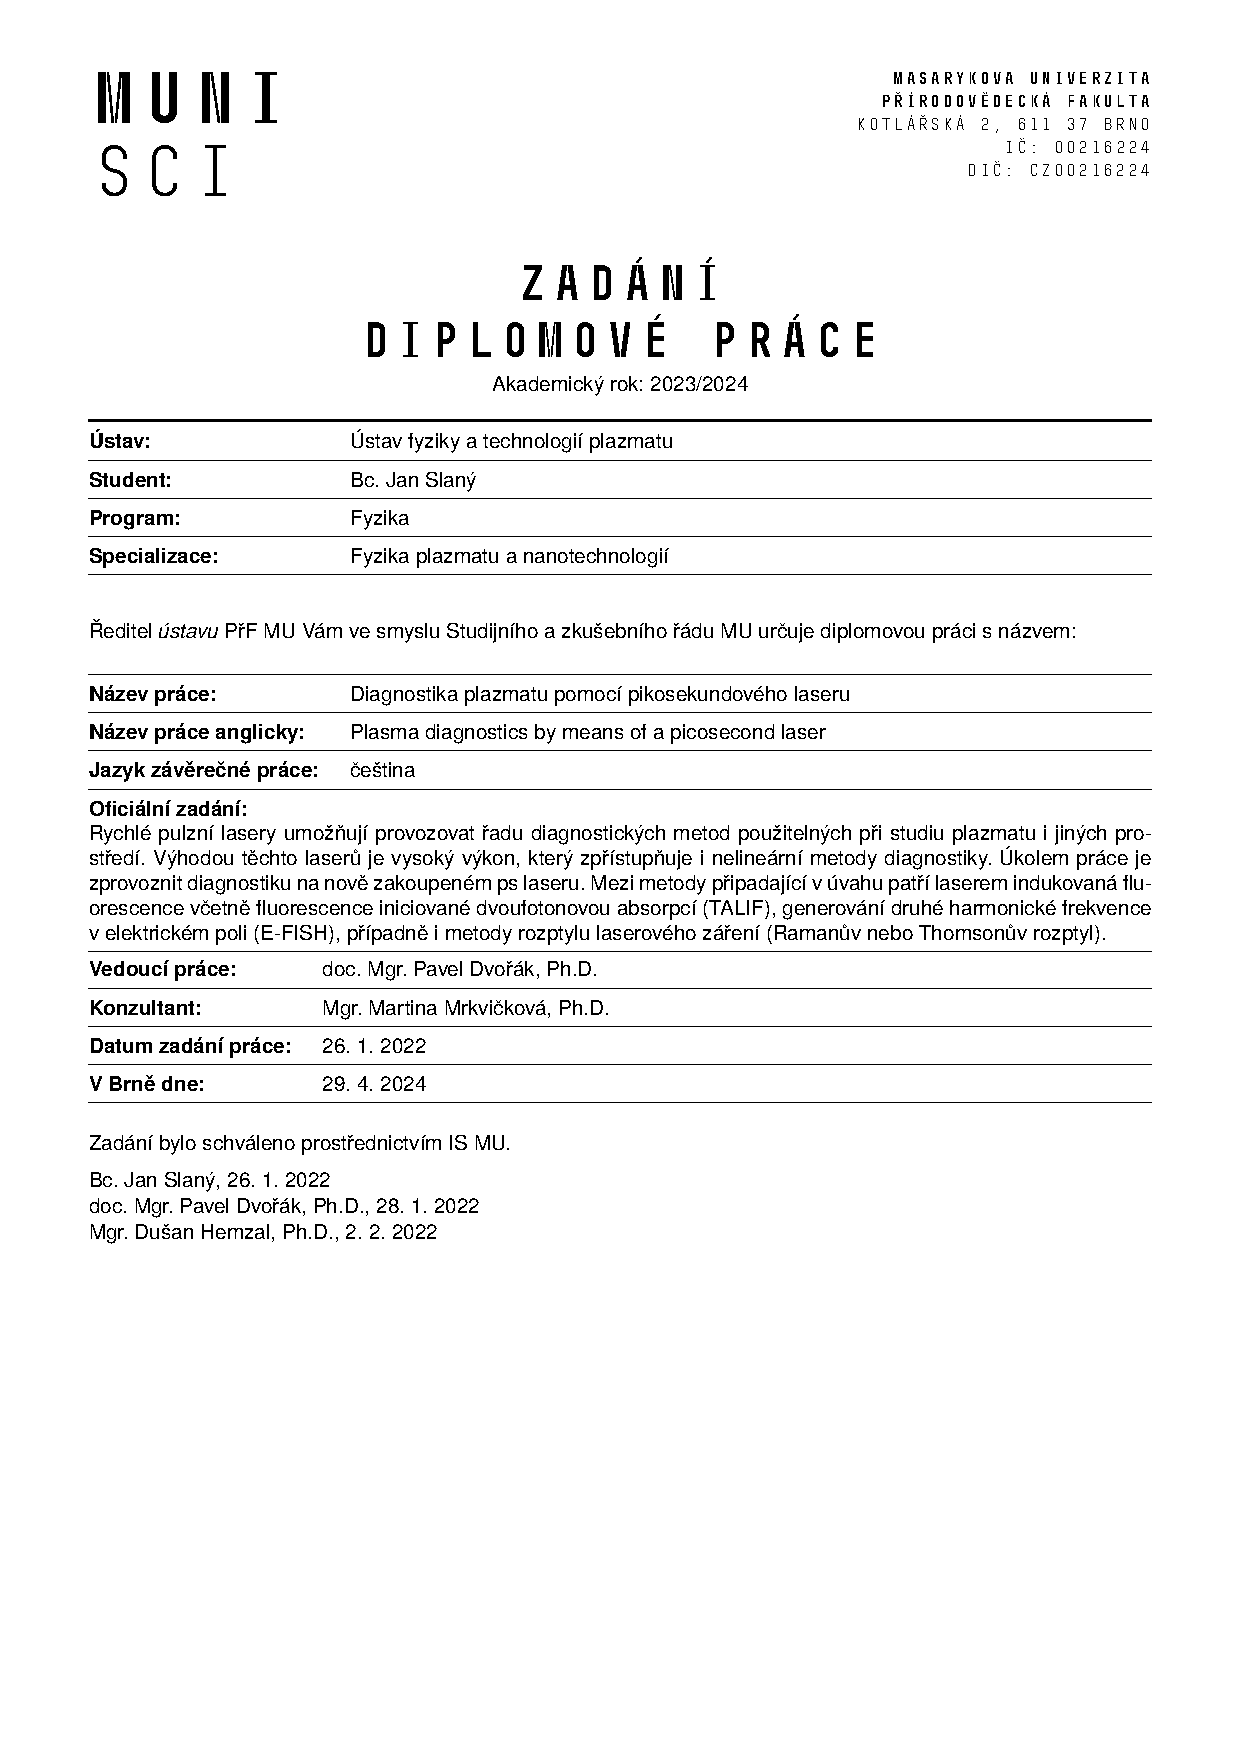
\includepdf[pages={1}]{../zadani.pdf}

% Acknowledgment
\chapter*{Poděkování}
% TODO: Poděkování
\vfill

% May be on the same page with acknowledgment
{\let\clearpage\relax\chapter*{Prohlášení}}
\thispagestyle{empty}
Prohlašuji, že jsem svou diplomovou práci vypracoval samostatně
pod vedením vedoucího práce s~využitím informačních zdrojů,
které jsou v~práci citovány.
\bigskip

\noindent
V Brně dne 27.~12.~2022 % TODO: Změnit datum
\hfill
\parbox{6cm}{
	\centering
	\vspace{1.5cm}
	\rule{6cm}{0.1pt}\par
	Jan Slaný
}
